%!TeX root=../tese.tex
%("dica" para o editor de texto: este arquivo é parte de um documento maior)
% para saber mais: https://tex.stackexchange.com/q/78101

\chapter{Ferramentas pedagógicas para ensino de Computação}
\label{related_tools}

Como vimos no Capítulo de Introdução, o ensino de Computação não está ligado a uma linguagem de programação específica, mas sim à abstração dos conceitos de programação e ao conjunto de habilidades que envolvem o pensamento computacional. Desse modo, diferentes ferramentas e tecnologias são utilizadas no apoio às aulas de Computação nas escolas. A seguir, discutimos algumas das abordagens mais utilizadas no ensino de programação para crianças e adolescentes.

\section{Linguagem de programação visual em blocos}

A linguagem de programação visual em blocos se baseia na construção de algoritmos usando blocos lógicos de maneira simples e intuitiva. Essa abordagem é amplamente utilizada em diversas ferramentas. Podemos citar como principal exemplo o \textit{Scratch} \citep{scratch2024}, uma plataforma, que utiliza uma linguagem de programação visual baseada em blocos e permite criar estórias, jogos e animações. Criada inicialmente por um grupo do \textit{MIT Media Lab} (Laboratório de Mídia do Instituto de Tecnologia de Massachusetts) e desenvolvida atualmente pela \textit{Scratch Foundation}, ela é uma ferramenta gratuita e de código aberto, e está disponível em mais de 70 idiomas. Segundo seus desenvolvedores, ela promove o pensamento educacional, habilidades de resolução de problemas, criatividade, auto-expressão, colaboração e equidade.

A Figura \ref{figure:sctrach} apresenta a interface do \textit{Scratch}. O espaço à esquerda permite arrastar os blocos das diferentes categorias à área central da página, onde é montado o algoritmo. À direita, temos o resultado da execução do conjunto de blocos apresentado na forma de animações.

\begin{figure}[h!]
    \centering
    \setlength{\fboxrule}{0.1pt} % espessura da borda da figura
    \fbox{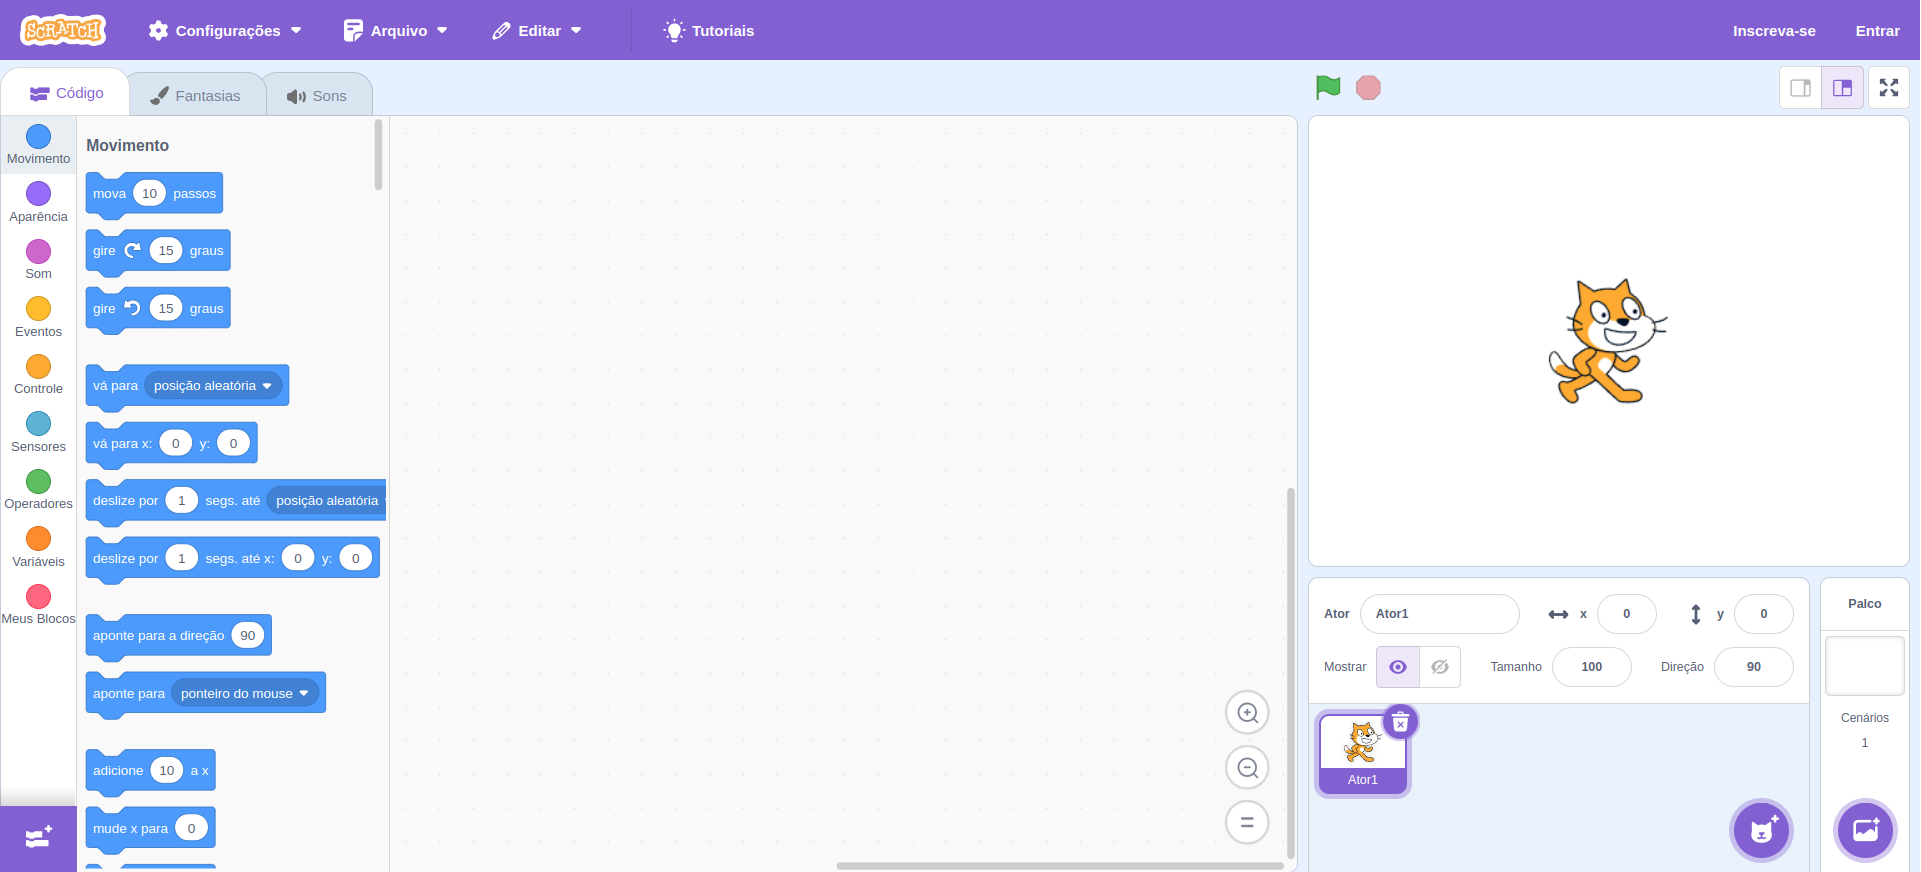
\includegraphics[scale=0.22]{scratch.png}}
    \caption{Interface do usuário da ferramenta \textit{Scratch} \citep{scratch2024}.}
    \label{figure:sctrach}
\end{figure}

Outra ferramenta baseada em blocos que merece destaque é o \textit{App Inventor} \citep{appinventor2024}, originalmente criado pelo Google e atualmente mantido pelo MIT. A plataforma permite a criação de aplicativos para os sistemas operacionais Android e iOS. Ela apresenta duas telas para a construção de um aplicativo: uma de design (Figura \ref{figure:app_inventor_design}), onde o visual do aplicativo pode ser montado, arrastando-se elementos visuais para a tela, como botões, texto de entrada, caixas de seleção, entres outros; e uma de blocos (Figura \ref{figure:app_inventor_logica}), onde é definida a lógica de interação com os elementos visuais adicionados como, por exemplo, qual efeito deve ser aplicado a um botão se ele for clicado.

\begin{figure}[t]
    \centering
    \setlength{\fboxrule}{0.1pt} % espessura da borda da figura
    \fbox{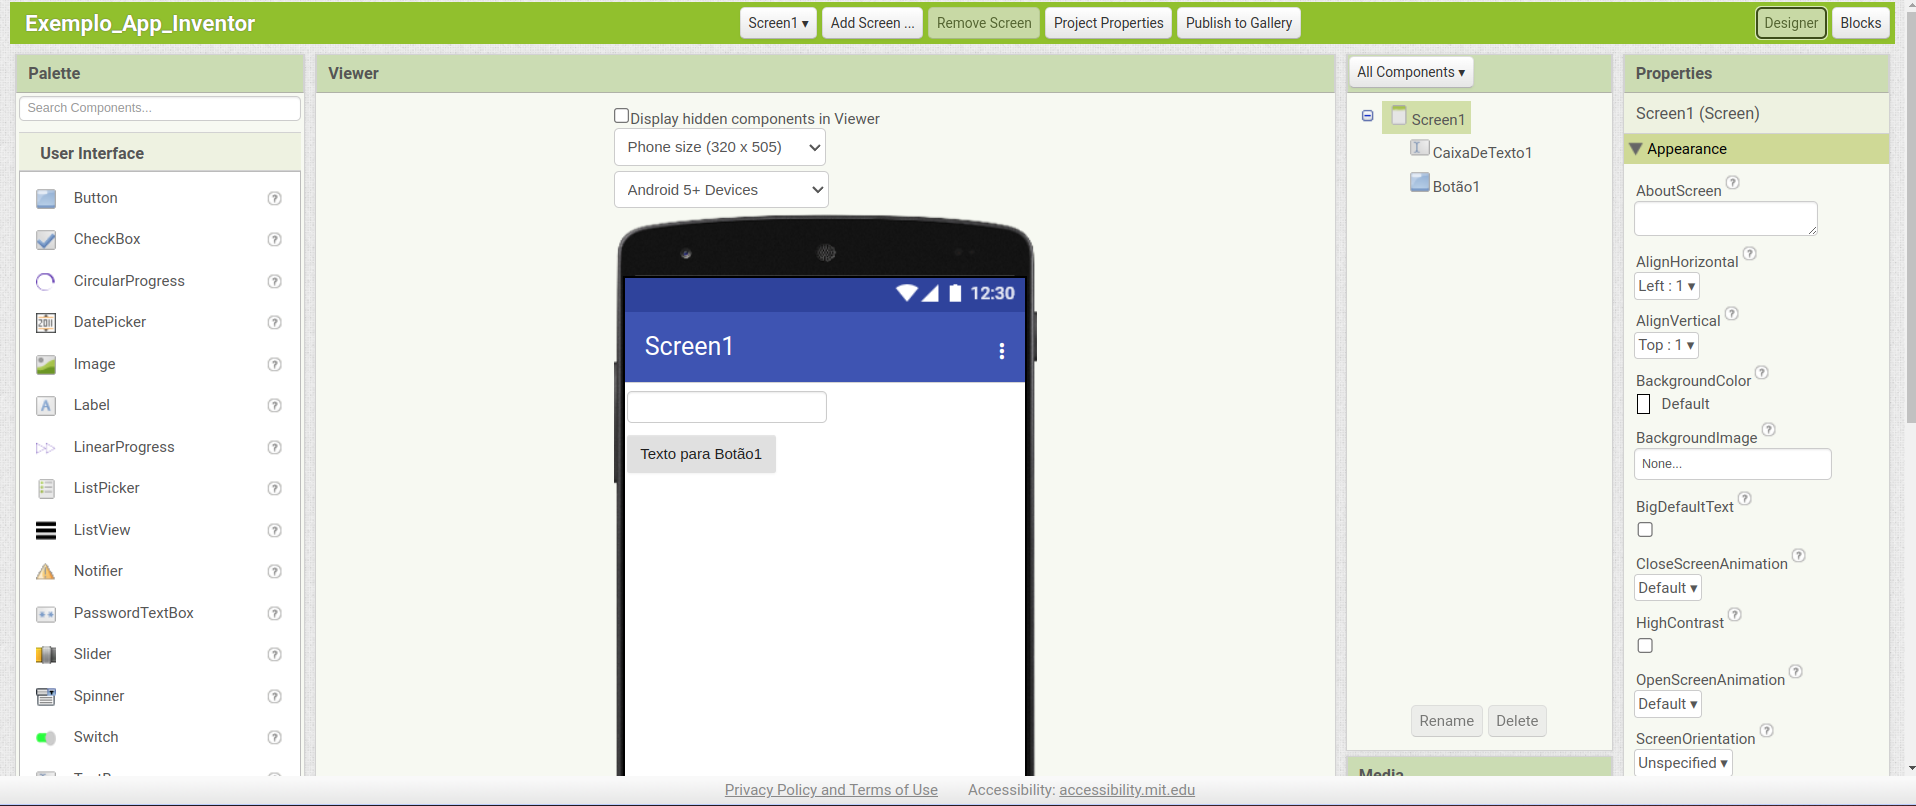
\includegraphics[scale=0.22]{figuras/app_inventor_design.png}}
    \caption{Interface do usuário da ferramenta \textit{App Inventor} para criar o design de um aplicativo \citep{appinventor2024}.}
    \label{figure:app_inventor_design}
\end{figure}

\begin{figure}[t]
    \centering
    \setlength{\fboxrule}{0.1pt} % espessura da borda da figura
    \fbox{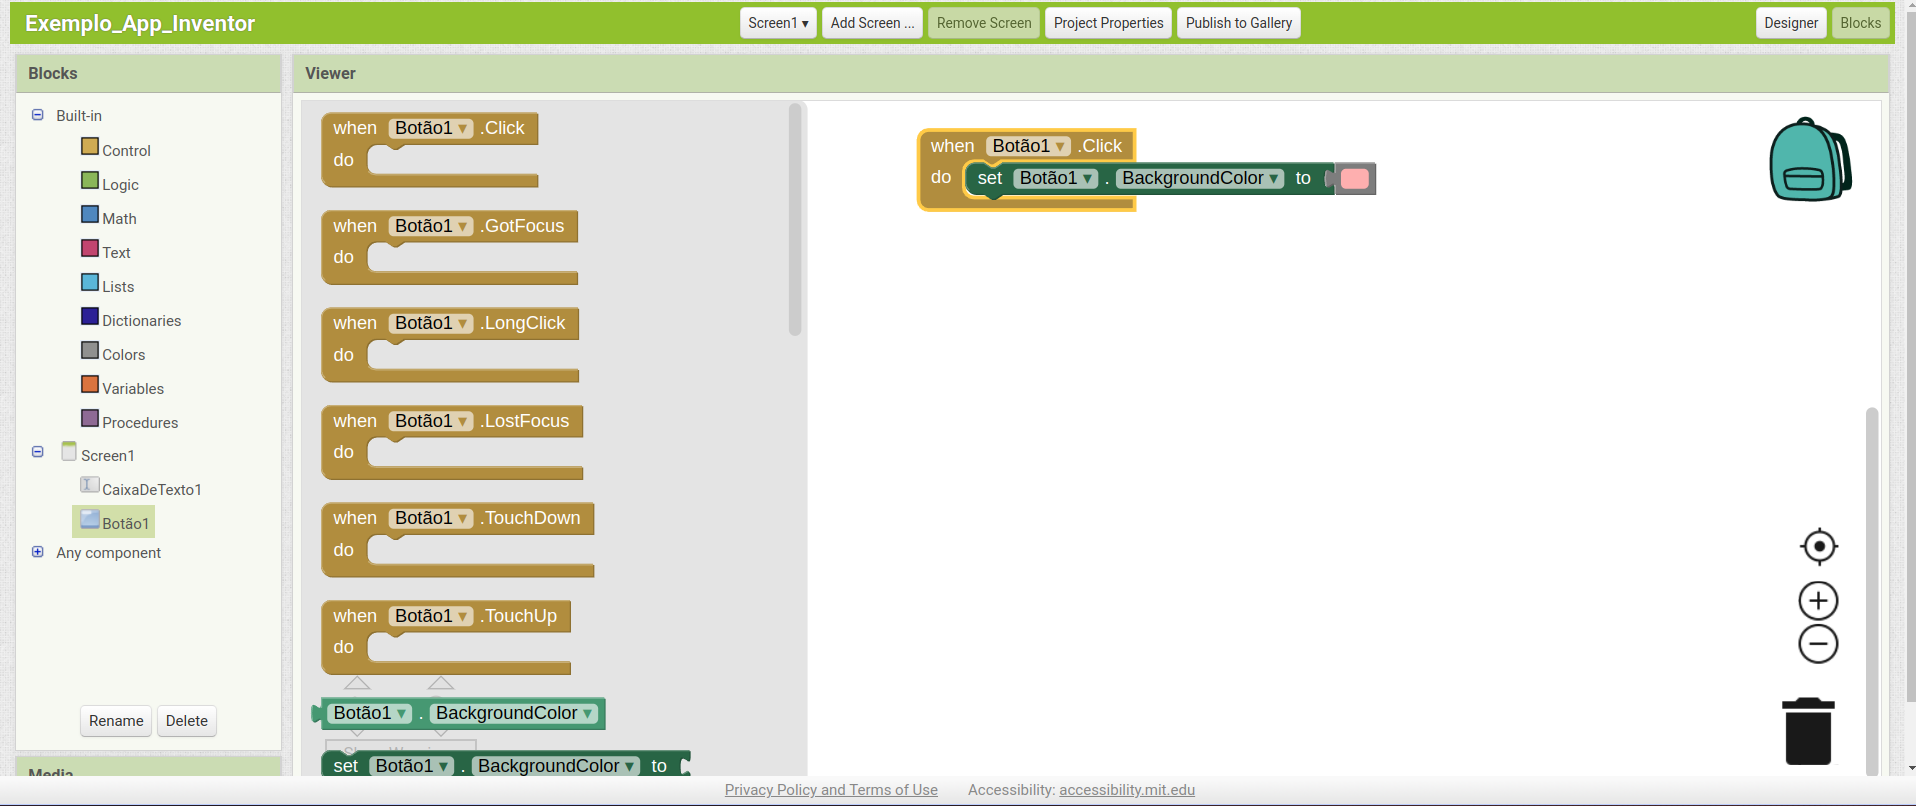
\includegraphics[scale=0.22]{figuras/app_inventor_logica.png}}
    \caption{Interface do usuário da ferramenta \textit{App Inventor} para criar a lógica de interação dos elementos do aplicativo \citep{appinventor2024}.}
    \label{figure:app_inventor_logica}
\end{figure}

Diversos estudos apontam esta abordagem, principalmente com o uso do \textit{Scratch}, como a mais utilizada no ensino de programação para crianças e adolescentes, apresentando resultados positivos \citep[e.g.][]{blatt2017mapeamento,bordini2016computaccao,khouri2020mapeamento,werlich2018pensamento}. Além disso, podemos observar que outras ferramentas, de jogos e robótica, por exemplo, também utilizam a linguagem visual em blocos em conjunto com sua metodologia principal. Alguns exemplos disso são: \textit{Blocky Games} \citep{blocklygames2024}, \textit{CodeCombat Junior} \citep{codecombat2024} e \textit{Lego Mindstorms} \citep{legomindstorms2024}.


\section{Jogos digitais}

A utilização de jogos digitais também pode estimular o pensamento computacional no ensino de programação. No geral, jogos fazem parte do cotidiano das crianças, além de aumentarem o engajamento e a motivação dos usuários. Um exemplo de jogo voltado para o ensino de programação é o \textit{CodeCombat} \citep{codecombat2024}, que permite que estudantes joguem e escrevam código utilizando uma linguagem baseada em texto com a sintaxe parecida com linguagens de programação. O jogo é gratuito e de código aberto, estando disponível em mais de 60 idiomas. Porém, a tradução para o português, muitas vezes, não é apresentada corretamente. A Figura \ref{figure:code_combate} apresenta a interface utilizada no \textit{CodeCombat}.

\begin{figure}[h!]
    \centering
    \setlength{\fboxrule}{0.1pt} % espessura da borda da figura
    \fbox{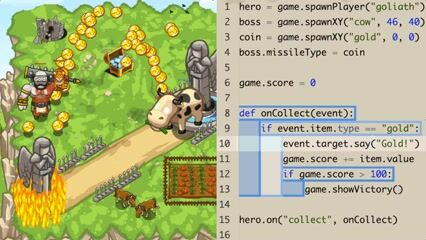
\includegraphics{figuras/code_combat.jpg}}
    \caption{Interface do usuário do jogo \textit{CodeCombat} \citep{codecombat2024}.}
    \label{figure:code_combate}
\end{figure}

Muitos desses jogos exploram comandos para orientar personagens, movendo-os para determinadas direções, e para realizar ações, utilizando de forma lúdica comandos com sintaxes muito similares a de funções das linguagens de programação.

\section{Kits de robótica}

Os kits de robótica combinam o uso de \textit{hardware} com o de software para o ensino de lógica de programação. A abordagem envolve a utilização de placas com microcontroladores e a montagem de circuitos ou robôs para realizarem determinadas tarefas como, por exemplo, um circuito ligado a lâmpadas de LED que poderão ser acesas ou um robô que irá andar alguns centímetros sobre o chão. O software, então, é utilizado para criar um programa que determina os comandos de execução dessas ações.

Um kit muito utilizado devido ao seu menor custo é o do Arduíno, que visa o controle de dispositivos, como LED e motores, ou a medição de variáveis, como temperatura e luminosidade. Ele requer conhecimentos em eletrônica por parte dos docentes e sua programação é feita através de um ambiente de desenvolvimento próprio baseado na linguagem de programação C \citep{klinczak2024estudo,demedeiros2019ensino}. Para facilitar a utilização deste tipo de ensino, algumas iniciativas criaram \textit{softwares} baseados na linguagem visual em blocos do \textit{Scratch} para escrever programas (Figura \ref{figure:arduino}).

\begin{figure}[h!]
    \centering
    \setlength{\fboxrule}{0.1pt} % espessura da borda da figura
    \fbox{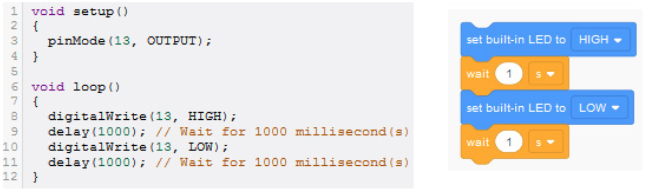
\includegraphics[scale=0.65]{figuras/arduino.png}}
    \caption{Exemplo da utilização da linguagem do \textit{Scratch} para programação do Arduíno \citep{demedeiros2019ensino}.}
    \label{figure:arduino}
\end{figure}

Outro exemplo com um custo mais elevado é o Kit educativo \textit{Lego Mindstorms}, o qual permite construir e programar um robô que pode andar, falar e pensar \citep{legomindstorms2024}. Sua montagem não requer conhecimentos de eletrônica, bastando apenas encaixar suas peças sem a necessidade de outras ferramentas (Figura \ref{figure:legomindstorms}). Também possui um ambiente próprio de programação visual, disponibilizado no site do fabricante.

\begin{figure}[h!]
    \centering
    \setlength{\fboxrule}{0.1pt} % espessura da borda da figura
    \fbox{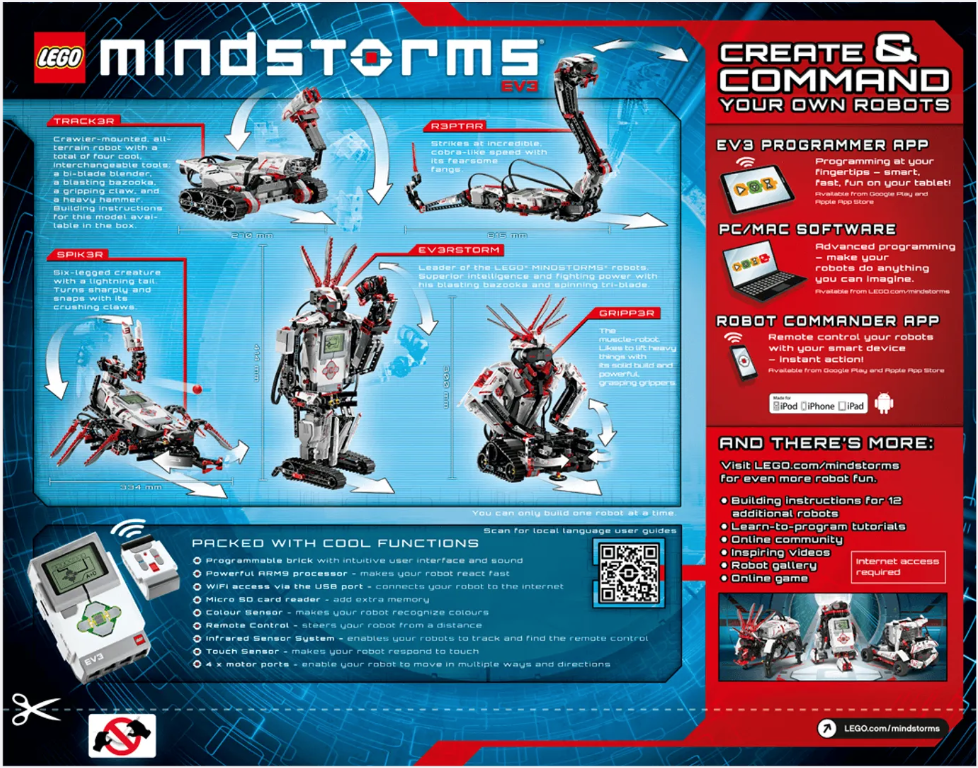
\includegraphics[scale=0.4]{figuras/lego_mindstorms.png}}
    \caption{Panorama o kit educativo \textit{Lego Mindstorms EV3} \citep{legomindstorms2024}.}
    \label{figure:legomindstorms}
\end{figure}

\section{Computação desplugada}

A Computação desplugada envolve atividades lúdicas que não necessitam do uso de computadores e podem abordar tópicos que ensinam conceitos de Computação, podendo ser realizadas por pessoas de quaisquer faixas etárias \citep{brackmann2017desenvolvimento}. Muitas vezes, as atividades envolvem ações de recortar, dobrar, colar, desenhar, pintar, resolver problemas, e os estudantes podem trabalhar em conjunto, promovendo habilidades de criatividade e colaboração. A Figura \ref{figure:desplugada} apresenta a descrição de um exemplo criado por \citet{brackmann2017desenvolvimento} em sua pesquisa sobre o desenvolvimento do pensamento computacional por meio de atividades desplugadas na educação básica.

\begin{figure}[h!]
    \centering
    \setlength{\fboxrule}{0.1pt} % espessura da borda da figura
    \fbox{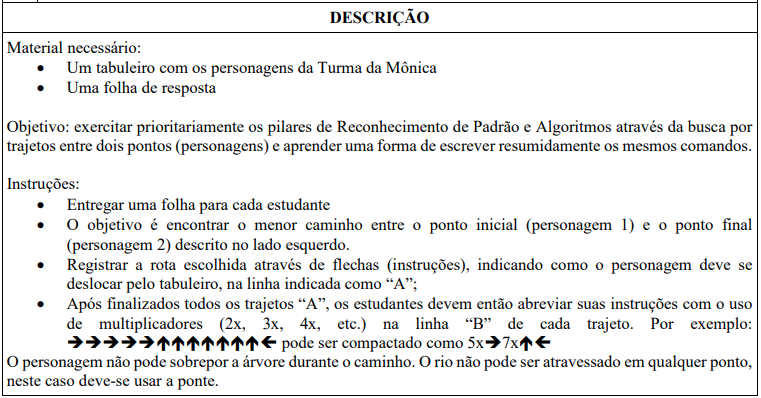
\includegraphics[scale=0.5]{figuras/desplugada.png}}
    \caption{Descrição de um exemplo de atividade desplugada \citep{brackmann2017desenvolvimento}.}
    \label{figure:desplugada}
\end{figure}

\section{Simulações interativas}

Simulações interativas utilizam elementos visuais do dia-a-dia para representar as abstrações envolvidas nos conceitos de diversas ciências, os quais não podemos ver ou manipular. Elas auxiliam no aprendizado desses tópicos, uma vez que os estudantes conseguem ver e manipular as interações \citep{price2018and}. Entretanto, ainda não existem muitas ferramentas que utilizem simulações interativas para o ensino de conceitos de lógica de programação. Em particular, não encontramos nenhuma ferramenta que se assemelhe a abordagem utilizada, de maneira bem-sucedida, pela plataforma PhET.

\citet{fernandes2012animacoes} criaram e avaliaram um objeto de aprendizagem na forma de animações e simulações no tema de variáveis de lógica de programação. O protótipo apresentava três partes: contextualização do conceito (sem interatividade), simulação de teste e fluxo de dados e uma atividade de fixação (Figura \ref{figure:oa}). Esse objeto de aprendizagem foi, então, avaliado por alunos e professores e os resultados obtidos demonstraram o potencial dessa abordagem. Porém, esse protótipo não foi encontrado disponível no link indicado no artigo.

\begin{figure}[h!]
    \centering
    \setlength{\fboxrule}{0.1pt} % espessura da borda da figura
    \fbox{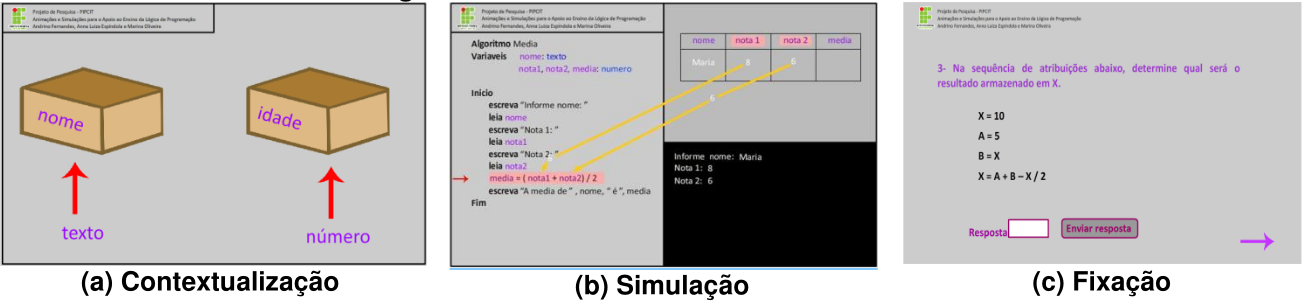
\includegraphics[scale=0.32]{figuras/objeto_aprendizagem.png}}
    \caption{Ilustração do objeto de aprendizagem de variáveis desenvolvido por \citet{fernandes2012animacoes}.}
    \label{figure:oa}
\end{figure}

Um outro exemplo encontrado, foi a ferramenta \textit{Drone Blocks} \citep{droneblocks2024}, um simulador de drones com programas projetados para o ensino de fundamentos de Ciência da Computação, entre outras finalidades não relacionadas a educação. A interface da simulação criada para o ensino (Figura \ref{figure:drone_blocks}) é muito similar a do \textit{Scratch}, a ferramenta utiliza a linguagem visual em blocos para construir instruções para o drone dentro de um cenário de sala de aula. Observamos como limitações dessa ferramenta o fato dela se restringir a simulações no contexto do drone na sala de aula e estar disponível apenas no idioma Inglês.

\begin{figure}[h!]
    \centering
    \setlength{\fboxrule}{0.1pt} % espessura da borda da figura
    \fbox{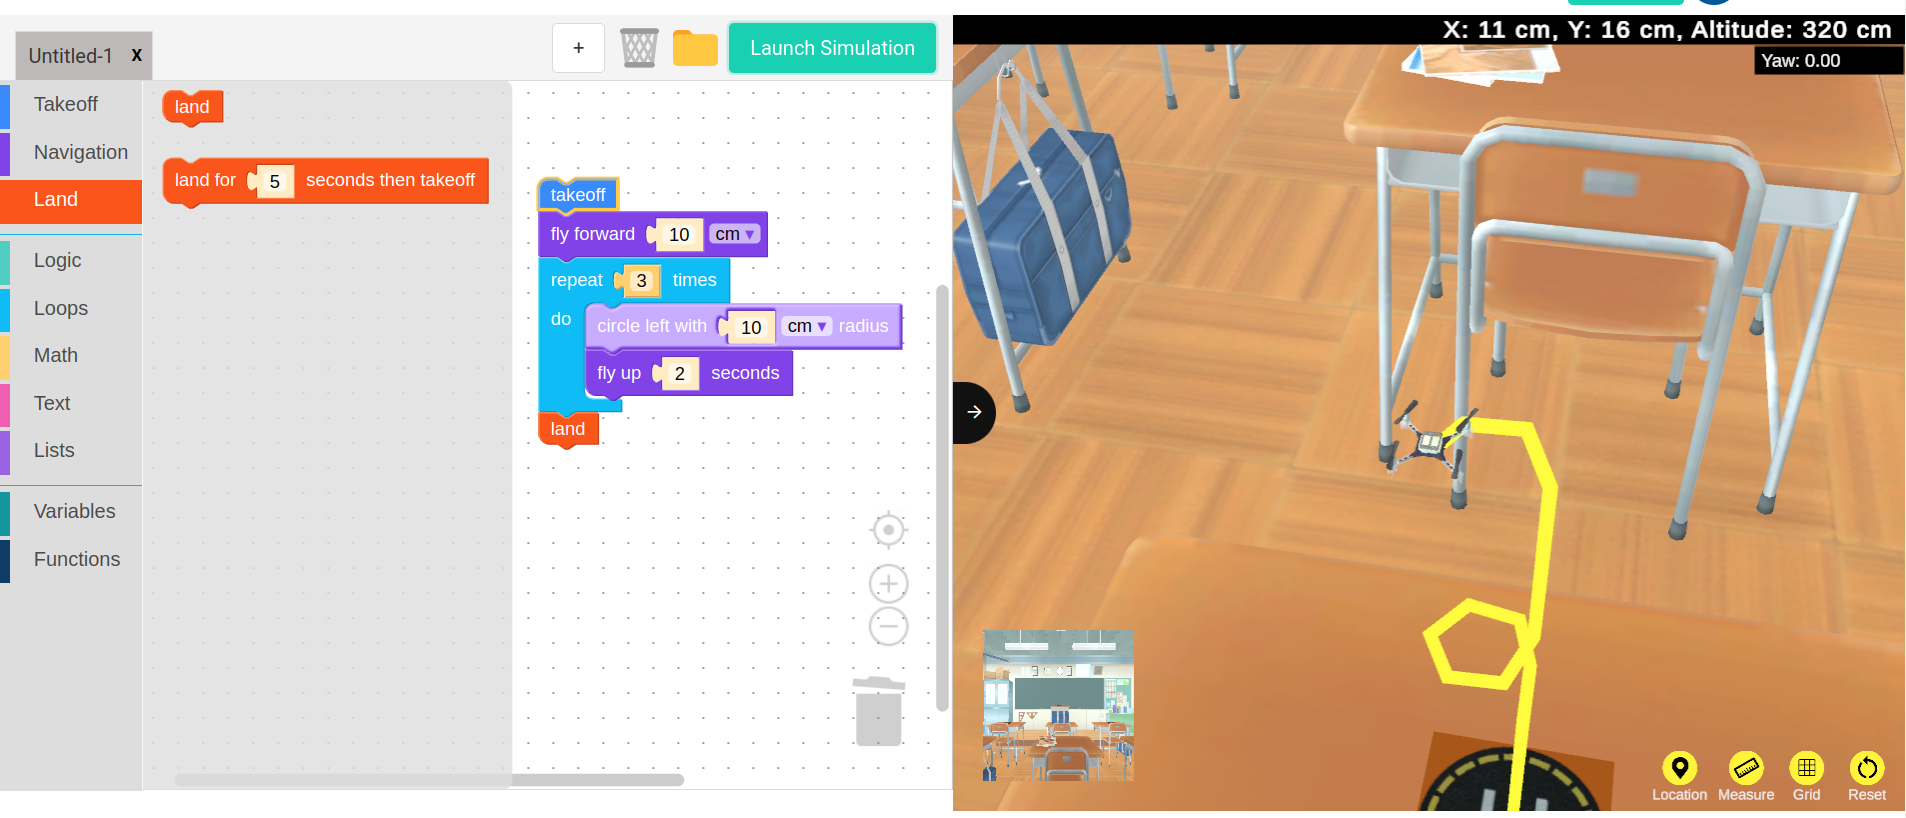
\includegraphics[scale=0.22]{figuras/drone_blocks.png}}
    \caption{Interface do usuário da simulação \textit{Drone Blocks} \citep{droneblocks2024}.}
    \label{figure:drone_blocks}
\end{figure}

Dessa maneira, o MVP proposto neste projeto tem um caráter inovador, uma vez que não foram encontradas, até o momento, outras ferramentas com propostas similares. Além disso, ele difere das demais abordagens apresentadas, pois na maioria delas o usuário constrói um código para visualizar a execução dele em forma de jogos, animações, histórias e aplicações. Já no protótipo proposto, há a interação com os elementos visuais da simulação e o pseudocódigo correspondente pode ser observado através dessas interações. Ainda, optamos por utilizar o pseudocódigo ao invés da linguagem de programação visual em blocos a fim de promover o contato com a estrutura real de um código fonte.